\documentclass[theme=teal]{khmermath}
\usepackage{needspace}
\geometry{left=0.9cm, right=0.9cm, top=0.85cm, bottom=1.80cm, footskip=0.90cm}
\usepackage{colortbl}
\usepackage{tikz}
\usetikzlibrary{calc,shapes,arrows,intersections,through,backgrounds,shadows,decorations.pathmorphing}

% Define arc accent
\newcommand{\wideparen}[1]{\overset{\boldsymbol{\frown}}{#1}}

% -------------------------------------------------------------------------
% Korean Math Textbook Style Color Palette & Macros
% -------------------------------------------------------------------------
\definecolor{koreaTeal}{RGB}{0, 150, 155}       % Primary Header Teal/Cyan
\definecolor{koreaDarkTeal}{RGB}{0, 105, 110}   % Dark Teal Accent
\definecolor{koreaBeige}{RGB}{247, 244, 237}     % Concept Sidebar Beige
\definecolor{koreaBeigeBorder}{RGB}{225, 218, 205}
\definecolor{koreaOrange}{RGB}{235, 115, 30}     % Problem Number Orange
\definecolor{koreaBlue}{RGB}{35, 110, 190}      % Standard Blue
\definecolor{koreaPurple}{RGB}{125, 50, 160}    % Purple Accent
\definecolor{koreaNumber}{RGB}{115, 125, 135}   % Problem Number Gray
\definecolor{koreaYellow}{RGB}{255, 246, 175}   % Yellow Highlight Tint

\definecolor{brandNavy}{RGB}{0, 105, 110}
\definecolor{brandBlue}{RGB}{0, 150, 155}
\definecolor{brandLightBlue}{RGB}{247, 244, 237}
\definecolor{brandCrimson}{RGB}{195, 35, 60}
\definecolor{brandCoral}{RGB}{235, 80, 75}
\definecolor{brandGold}{RGB}{215, 130, 10}
\definecolor{brandGoldBg}{RGB}{255, 252, 242}
\definecolor{brandOrange}{RGB}{235, 115, 30}
\definecolor{brandTeal}{RGB}{0, 150, 155}
\definecolor{brandTealBg}{RGB}{244, 252, 250}
\definecolor{subtleGray}{RGB}{246, 251, 249}
\definecolor{cardBorder}{RGB}{220, 212, 198}
\definecolor{solidFill}{RGB}{238, 248, 248}
\definecolor{solidDarkFill}{RGB}{215, 238, 238}

% Custom Header & Footer setup (Korean Textbook Style with safe spacing)
\usepackage{fancyhdr}
\pagestyle{fancy}
\fancyhf{}
\renewcommand{\headrulewidth}{0pt}
\renewcommand{\footrule}{\color{koreaTeal!60}\hrule height 0.6pt\vspace{3.5pt}}

\fancyfoot[L]{%
  \fontsize{8.5}{8.5}\selectfont\kml \color{koreaNumber}\textbf{\thepage}\ \vline\ \color{koreaDarkTeal}\textbf{១៨. សូលីត}%
}
\fancyfoot[C]{%
  \fontsize{8.5}{8.5}\selectfont\kby \color{koreaDarkTeal}\textbf{\ding{72}\ បង្រៀនដោយ ៖ \textcolor{koreaDarkTeal}{ក្រូត រស្មី}\ \ding{72}}%
}
\fancyfoot[R]{%
  \fontsize{8.5}{8.5}\selectfont\kby \color{koreaDarkTeal}\textbf{ Telegram: \textcolor{brandCrimson}{070897540}}\ \vline\ \color{koreaNumber}\textbf{\thepage}%
}

% Korean Header Banner (Only on Page 1)
\newcommand{\koreanheader}[2]{%
  \noindent%
  \begin{tikzpicture}[x=1cm, y=1cm]
    \fill[koreaTeal, rounded corners=12pt] (0, 0.1) -- (0, 0.95) -- (3.8, 0.95) [rounded corners=0pt] -- (4.4, 0.1) -- cycle;
    \node[white, font=\fontsize{11}{11}\selectfont\kml\bfseries] at (1.9, 0.52) {#1};
    \node[anchor=west, font=\fontsize{16}{16}\selectfont\kml\bfseries, color=koreaDarkTeal] at (4.6, 0.42) {#2};
    \node[anchor=east, font=\fontsize{8.5}{8.5}\selectfont\kby, color=gray!80] at (19.2, 0.48) {$>$ ក្លឹបសិក្សាគណិតវិទ្យា ភី ស៊ី​ អឹម};
  \end{tikzpicture}%
  \vspace{1pt}%
}

% Yellow Formula Highlight Box
\newcommand{\koreahl}[1]{\colorbox{koreaYellow}{\fontsize{8.5}{8.5}\selectfont\textbf{#1}}}

% General Rule Box (Teal/Navy Theme - ជាទូទៅ)
\newtcolorbox{khboxorange}[1][]{
  enhanced,
  colframe=brandNavy!40,
  colback=brandLightBlue,
  boxrule=0.7pt,
  arc=4.5pt,
  borderline west={3.5pt}{0pt}{brandNavy},
  drop fuzzy shadow=brandNavy!15,
  left=7pt, right=7pt, top=3pt, bottom=2.5pt,
  title={\fontsize{9}{9}\selectfont\kml\color{white}\ding{72}\ ជាទូទៅ},
  coltitle=white,
  colbacktitle=brandNavy,
  boxed title style={
    boxrule=0pt,
    arc=3pt,
    left=6pt, right=6pt, top=2pt, bottom=2pt
  },
  attach boxed title to top left={yshift*=-\tcboxedtitleheight/2, xshift=10pt},
  #1
}

% Concept / Card Item Box
\newtcolorbox{khcard}[1][]{
  enhanced,
  colframe=cardBorder,
  colback=white,
  boxrule=0.6pt,
  arc=3.5pt,
  left=6pt, right=6pt, top=4pt, bottom=4pt,
  #1
}

% Section, Subsection & Header Badge Macros
\newcommand{\khsection}[2]{%
  \par\needspace{2.8cm}%
  \vspace{6pt}%
  \noindent%
  \begin{tikzpicture}
    \fill[rounded corners=4pt, brandNavy!8] (0,0) rectangle (19.2, 0.60);
    \fill[rounded corners=3pt, brandNavy] (0.05, 0.05) rectangle (0.55, 0.55);
    \node[white, font=\fontsize{9.5}{9.5}\selectfont\bfseries] at (0.30, 0.30) {#1};
    \fill[brandGold, rounded corners=1pt] (0.65, 0.12) rectangle (0.69, 0.48);
    \node[anchor=west, font=\fontsize{10.5}{10.5}\selectfont\kml, color=brandCrimson] at (0.75, 0.30) {\textbf{#2}};
  \end{tikzpicture}%
  \par\vspace{3pt}%
}

\newcommand{\khsubsection}[2]{%
  \par\needspace{2.2cm}%
  \vspace{3.5pt}%
  \noindent%
  \begin{tikzpicture}[baseline=(sub.base)]
    \node[rounded corners=3pt, fill=brandBlue!12, draw=brandBlue!35, line width=0.5pt, text=brandNavy, font=\fontsize{8.5}{8.5}\selectfont\kml\bfseries, inner sep=2.2pt] (sub) at (0,0) {#1};
    \node[anchor=west, font=\fontsize{9.5}{9.5}\selectfont\kml\bfseries, color=brandNavy] at (sub.east) {\ \ #2};
  \end{tikzpicture}%
  \par\vspace{2pt}%
}

\def\splitnum#1#2{%
  \color{koreaNumber!65}#1\color{koreaOrange}#2%
}
\newcommand{\koreannum}[1]{%
  \ifstrempty{#1}{}{%
    \mbox{%
      \fontsize{15}{15}\selectfont\bfseries%
      \ifnum#1<10\relax%
        \color{koreaNumber!65}0\color{koreaOrange}#1%
      \else%
        \expandafter\splitnum#1%
      \fi%
    }\,\ %
  }%
}

% Khmer Sub-item Badge (ក, ខ, គ)
\newcommand{\khlabel}[1]{%
  \tikz[baseline=-0.6ex]{%
    \node[fill=brandCrimson, rounded corners=2.8pt, inner sep=1.8pt, minimum width=1.25em, minimum height=1.25em, text=white, font=\kml\fontsize{7.5}{7.5}\selectfont, align=center] (lbl) {\raisebox{0.2pt}{#1}};%
  }\,\ %
}

% Styled Exercise Head (01, 02, 03...)
\newcommand{\exhead}[1]{%
  \koreannum{#1}%
}

% 2-Column Aligned Items helper
\newcommand{\itemtwo}[2]{%
  \noindent\makebox[0.485\linewidth][l]{#1}\hfill\makebox[0.485\linewidth][l]{#2}\par\vspace{1.5pt}%
}

% Setup column separator in multicols
\setlength{\columnsep}{16pt}
\setlength{\columnseprule}{0.35pt}
\def\columnseprulecolor{\color{brandNavy!20}}

\begin{document}

% =========================================================================
% មេរៀនទី ១៨ ៖ សូលីត (Header on Page 1 Only)
% =========================================================================
\koreanheader{មេរៀនទី ១៨}{សូលីត}

\khsection{១}{ផ្ទៃក្រឡានិងមាឌនៃសូលីត}

\khsubsection{១.១}{ផ្ទៃក្រឡាខាង និងផ្ទៃក្រឡាទាំងអស់នៃសូលីត}

\begin{khcard}
  \begin{minipage}[t]{0.48\linewidth}
    \textbf{\color{brandNavy}\ding{70} ធាតុសំខាន់ៗនៃកោន (Cone) ៖}
    \vspace{-2pt}
    \begin{center}
      \begin{tikzpicture}[scale=0.68]
        \draw[thick, color=brandNavy] (-1.4, 0) arc (180:360:1.4cm and 0.42cm);
        \draw[dashed, color=brandNavy!60] (-1.4, 0) arc (180:0:1.4cm and 0.42cm);
        \draw[thick, color=brandNavy] (-1.4, 0) -- (0, 2.3) node[above, font=\fontsize{8}{8}\selectfont, color=brandNavy] {$S$};
        \draw[thick, color=brandNavy] (1.4, 0) -- (0, 2.3);
        \coordinate (O) at (0,0);
        \coordinate (S) at (0,2.3);
        \draw[dashed, color=brandCrimson, thick] (S) -- (O) node[midway, left=-1pt, font=\fontsize{7.5}{7.5}\selectfont] {កម្ពស់ $h$};
        \draw[dashed, color=brandBlue, thick] (O) -- (1.4, 0) node[midway, below=-1pt, font=\fontsize{7.5}{7.5}\selectfont] {កាំ $R$};
        \node[right=1pt, font=\fontsize{7.5}{7.5}\selectfont, color=brandNavy] at (0.7, 1.25) {ជេនេត្រ $a$};
        \fill[brandCrimson] (O) circle (1.2pt) node[below=1pt, font=\fontsize{7}{7}\selectfont] {$O$};
        \draw[color=brandCrimson] (0, 0.16) -- (0.16, 0.16) -- (0.16, 0);
        \node[below, font=\fontsize{7.5}{7.5}\selectfont, color=brandNavy] at (0, -0.5) {បាតជារង្វង់};
      \end{tikzpicture}
    \end{center}
  \end{minipage}
  \hfill
  \begin{minipage}[t]{0.48\linewidth}
    \textbf{\color{brandNavy}\ding{70} ធាតុសំខាន់ៗនៃពីរ៉ាមីតនិយ័ត (Pyramid) ៖}
    \vspace{-2pt}
    \begin{center}
      \begin{tikzpicture}[scale=0.68]
        \coordinate (S) at (0, 2.3);
        \coordinate (A) at (-1.4, -0.3);
        \coordinate (B) at (-0.6, -0.7);
        \coordinate (C) at (0.6, -0.7);
        \coordinate (D) at (1.4, -0.3);
        \coordinate (E) at (0.7, 0.15);
        \coordinate (F) at (-0.7, 0.15);
        \coordinate (O) at (0, -0.2);
        \coordinate (H) at (0, -0.7);
        
        \draw[dashed, color=gray!70] (A) -- (F) -- (E) -- (D);
        \draw[dashed, color=gray!70] (S) -- (F);
        \draw[dashed, color=gray!70] (S) -- (E);
        \draw[dashed, color=brandCrimson, thick] (S) -- (O) node[midway, left=-1pt, font=\fontsize{7.5}{7.5}\selectfont] {កម្ពស់ $h$};
        \draw[dashed, color=brandOrange, thick] (S) -- (H) node[midway, right=1pt, font=\fontsize{7.5}{7.5}\selectfont] {អាប៉ូតែម $a$};
        
        \draw[thick, color=brandNavy] (A) -- (B) -- (C) -- (D);
        \draw[thick, color=brandNavy] (S) -- (A);
        \draw[thick, color=brandNavy] (S) -- (B);
        \draw[thick, color=brandNavy] (S) -- (C);
        \draw[thick, color=brandNavy] (S) -- (D);
        
        \fill[brandCrimson] (O) circle (1.2pt) node[below=1pt, font=\fontsize{7}{7}\selectfont] {$O$};
        \node[above, font=\fontsize{8}{8}\selectfont, color=brandNavy] at (S) {$S$ (កំពូល)};
        \node[below, font=\fontsize{7.5}{7.5}\selectfont, color=brandNavy] at (0, -0.8) {បាតជាពហុកោណនិយ័ត};
      \end{tikzpicture}
    \end{center}
  \end{minipage}
  \vspace{-2pt}
  \begin{center}
    \fontsize{8}{8}\selectfont\textbf{\color{brandNavy}ប្រភេទពីរ៉ាមីតនិយ័ត ៖} បាតជាត្រីកោណសម័ង្ស ($ABC$), បាតជាការេ ($ABCD$) និង បាតជាឆកោណនិយ័ត ($ABCDEF$)
  \end{center}
\end{khcard}

\begin{khboxorange}
  \begin{itemize}[leftmargin=12pt, itemsep=1.5pt, topsep=1pt, parsep=0pt]
    \item[\color{brandNavy}\ding{228}] \textbf{ផ្ទៃក្រឡាខាងនៃពីរ៉ាមីតនិយ័ត ៖} \koreahl{$S_L = \frac{1}{2} \times p \times a$} \quad \text{($p$ ជាបរិមាត្របាត, $a$ ជាអាប៉ូតែម)}
    \item[\color{brandNavy}\ding{228}] \textbf{ផ្ទៃក្រឡាទាំងអស់នៃពីរ៉ាមីត ៖} \koreahl{$S_T = S_L + S_B$} \quad \text{($S_B$ ជាផ្ទៃក្រឡាបាត)}
    \item[\color{brandCrimson}\ding{228}] \textbf{ផ្ទៃក្រឡាខាងនៃកោន ៖} \koreahl{$S_L = \pi R a$} \quad \text{($R$ ជាកាំបាត, $a$ ជាប្រវែងជេនេត្រ)}
    \item[\color{brandCrimson}\ding{228}] \textbf{ផ្ទៃក្រឡាទាំងអស់នៃកោន ៖} \koreahl{$S_T = S_L + S_B = \pi R a + \pi R^2 = \pi R(a + R)$}
  \end{itemize}
\end{khboxorange}

\begin{multicols}{2}
  % [ស្រួល - Direct formulas]
  \noindent\begin{minipage}{\linewidth}
    \exhead{1} គណនាផ្ទៃក្រឡាខាងនៃពីរ៉ាមីតនិយ័តដែលមានបាតរាងជាការេមានជ្រុង $3\text{cm}$ និងអាប៉ូតែម $4\text{cm}$ ។
  \end{minipage}\par\vspace{5pt}

  \noindent\begin{minipage}{\linewidth}
    \exhead{2} គណនាផ្ទៃក្រឡាខាងនៃពីរ៉ាមីតនិយ័តដែលមានបាតជាឆកោណនិយ័តជ្រុង $6\text{cm}$ និងអាប៉ូតែម $7\text{cm}$ ។
    \begin{center}
      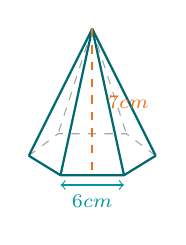
\begin{tikzpicture}[scale=0.62]
        \coordinate (S) at (0, 2.3);
        \coordinate (A) at (-1.3, -0.3);
        \coordinate (B) at (-0.65, -0.7);
        \coordinate (C) at (0.65, -0.7);
        \coordinate (D) at (1.3, -0.3);
        \coordinate (E) at (0.7, 0.15);
        \coordinate (F) at (-0.7, 0.15);
        \coordinate (H) at (0, -0.7);
        \draw[dashed, color=gray!70] (A) -- (F) -- (E) -- (D);
        \draw[dashed, color=gray!70] (S) -- (F);
        \draw[dashed, color=gray!70] (S) -- (E);
        \draw[thick, color=brandNavy] (A) -- (B) -- (C) -- (D);
        \draw[thick, color=brandNavy] (S) -- (A);
        \draw[thick, color=brandNavy] (S) -- (B);
        \draw[thick, color=brandNavy] (S) -- (C);
        \draw[thick, color=brandNavy] (S) -- (D);
        \draw[dashed, color=brandOrange, thick] (S) -- (H) node[midway, right=2pt, font=\fontsize{7.5}{7.5}\selectfont] {$7\text{cm}$};
        \draw[<->, color=brandBlue, font=\fontsize{7.5}{7.5}\selectfont] (-0.65, -0.9) -- (0.65, -0.9) node[midway, below] {$6\text{cm}$};
      \end{tikzpicture}
    \end{center}
  \end{minipage}\par\vspace{5pt}

  \noindent\begin{minipage}{\linewidth}
    \exhead{3} គណនាផ្ទៃក្រឡាទាំងអស់នៃពីរ៉ាមីតនិយ័តបាតការេជ្រុង $15\text{cm}$ និងអាប៉ូតែម $12\text{cm}$ ។
    \begin{center}
      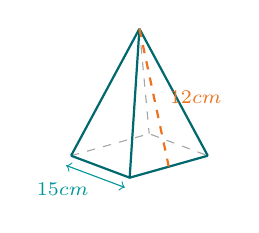
\begin{tikzpicture}[scale=0.62]
        \coordinate (S) at (0, 2.3);
        \coordinate (A) at (-1.4, -0.3);
        \coordinate (B) at (-0.2, -0.75);
        \coordinate (C) at (1.4, -0.3);
        \coordinate (D) at (0.2, 0.15);
        \coordinate (H) at (0.6, -0.52);
        \draw[dashed, color=gray!70] (A) -- (D) -- (C);
        \draw[dashed, color=gray!70] (S) -- (D);
        \draw[thick, color=brandNavy] (A) -- (B) -- (C);
        \draw[thick, color=brandNavy] (S) -- (A);
        \draw[thick, color=brandNavy] (S) -- (B);
        \draw[thick, color=brandNavy] (S) -- (C);
        \draw[dashed, color=brandOrange, thick] (S) -- (H) node[midway, right=2pt, font=\fontsize{7.5}{7.5}\selectfont] {$12\text{cm}$};
        \draw[<->, color=brandBlue, font=\fontsize{7.5}{7.5}\selectfont] (-1.5, -0.5) -- (-0.3, -0.95) node[midway, below left=-1pt] {$15\text{cm}$};
      \end{tikzpicture}
    \end{center}
  \end{minipage}\par\vspace{5pt}

  % [មធ្យម - Cone & multi-part problems]
  \noindent\begin{minipage}{\linewidth}
    \exhead{4} គណនាផ្ទៃក្រឡាខាង និងផ្ទៃក្រឡាទាំងអស់នៃកោនដែលមានកាំបាត $4\text{cm}$ និងជេនេត្រ $13\text{cm}$ (យក $\pi = 3.14$) ។
    \begin{center}
      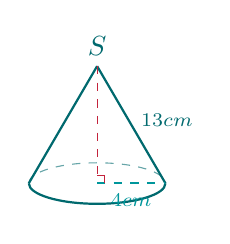
\begin{tikzpicture}[scale=0.62]
        \draw[thick, color=brandNavy] (-1.4, 0) arc (180:360:1.4cm and 0.42cm);
        \draw[dashed, color=brandNavy!60] (-1.4, 0) arc (180:0:1.4cm and 0.42cm);
        \draw[thick, color=brandNavy] (-1.4, 0) -- (0, 2.4) node[above, color=brandNavy] {$S$};
        \draw[thick, color=brandNavy] (1.4, 0) -- (0, 2.4);
        \coordinate (O) at (0,0);
        \coordinate (S) at (0,2.4);
        \draw[dashed, color=brandCrimson] (S) -- (O);
        \draw[dashed, color=brandBlue, thick] (O) -- (1.4, 0) node[midway, below, font=\fontsize{7.5}{7.5}\selectfont] {$4\text{cm}$};
        \node[right, font=\fontsize{7.5}{7.5}\selectfont, color=brandNavy] at (0.7, 1.3) {$13\text{cm}$};
        \draw[color=brandCrimson] (0, 0.16) -- (0.16, 0.16) -- (0.16, 0);
      \end{tikzpicture}
    \end{center}
  \end{minipage}\par\vspace{5pt}

  \noindent\begin{minipage}{\linewidth}
    \exhead{5} ចូរគណនាផ្ទៃក្រឡាខាង និងផ្ទៃក្រឡាទាំងអស់នៃរូបខាងក្រោម ៖
    \begin{itemize}[leftmargin=14pt, labelsep=3pt, itemsep=1.5pt]
      \item[\khlabel{ក}] ពីរ៉ាមីតបាតការេជ្រុង $5\text{cm}$ អាប៉ូតែម $13\text{cm}$
      \item[\khlabel{ខ}] កោនមានកាំបាត $5\text{cm}$ ជេនេត្រ $10\text{cm}$
      \item[\khlabel{គ}] ពីរ៉ាមីតបាតឆកោណនិយ័តជ្រុង $2\text{cm}$ អាប៉ូតែម $5\text{cm}$
    \end{itemize}
  \end{minipage}\par\vspace{5pt}

  % [ពិបាក - Multi-solid diagrams: perfectly aligned on baseline using minipages]
  \noindent\begin{minipage}{\linewidth}
    \exhead{6} ចូររកផ្ទៃក្រឡាខាង និងផ្ទៃក្រឡាទាំងអស់នៃរូបខាងក្រោម ៖
    \begin{center}
      \vspace{-3pt}
      \begin{minipage}[t]{0.32\linewidth}
        \centering
        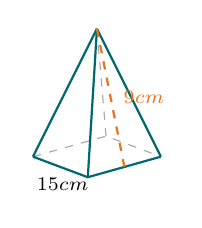
\begin{tikzpicture}[scale=0.58]
          \coordinate (S) at (0, 2.5);
          \coordinate (A) at (-1.4, -0.3);
          \coordinate (B) at (-0.2, -0.75);
          \coordinate (C) at (1.4, -0.3);
          \coordinate (D) at (0.2, 0.15);
          \coordinate (H) at (0.6, -0.52);
          \draw[dashed, color=gray!70] (A) -- (D) -- (C);
          \draw[dashed, color=gray!70] (S) -- (D);
          \draw[thick, color=brandNavy] (A) -- (B) -- (C);
          \draw[thick, color=brandNavy] (S) -- (A);
          \draw[thick, color=brandNavy] (S) -- (B);
          \draw[thick, color=brandNavy] (S) -- (C);
          \draw[dashed, color=brandOrange, thick] (S) -- (H) node[midway, right=1pt, font=\fontsize{7.5}{7.5}\selectfont] {$9\text{cm}$};
          \node[below, font=\fontsize{7.5}{7.5}\selectfont] at (-0.75, -0.55) {$15\text{cm}$};
        \end{tikzpicture}\par\vspace{2pt}
        \khlabel{ក}
      \end{minipage}\hfill
      \begin{minipage}[t]{0.32\linewidth}
        \centering
        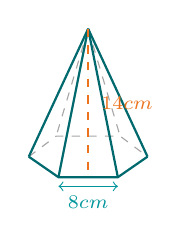
\begin{tikzpicture}[scale=0.58]
          \coordinate (S) at (0, 2.5);
          \coordinate (A) at (-1.3, -0.3);
          \coordinate (B) at (-0.65, -0.75);
          \coordinate (C) at (0.65, -0.75);
          \coordinate (D) at (1.3, -0.3);
          \coordinate (E) at (0.7, 0.15);
          \coordinate (F) at (-0.7, 0.15);
          \coordinate (H) at (0, -0.75);
          \draw[dashed, color=gray!70] (A) -- (F) -- (E) -- (D);
          \draw[dashed, color=gray!70] (S) -- (F);
          \draw[dashed, color=gray!70] (S) -- (E);
          \draw[thick, color=brandNavy] (A) -- (B) -- (C) -- (D);
          \draw[thick, color=brandNavy] (S) -- (A);
          \draw[thick, color=brandNavy] (S) -- (B);
          \draw[thick, color=brandNavy] (S) -- (C);
          \draw[thick, color=brandNavy] (S) -- (D);
          \draw[dashed, color=brandOrange, thick] (S) -- (H) node[midway, right=1pt, font=\fontsize{7.5}{7.5}\selectfont] {$14\text{cm}$};
          \draw[<->, color=brandBlue, font=\fontsize{7.5}{7.5}\selectfont] (-0.65, -0.95) -- (0.65, -0.95) node[midway, below] {$8\text{cm}$};
        \end{tikzpicture}\par\vspace{2pt}
        \khlabel{ខ}
      \end{minipage}\hfill
      \begin{minipage}[t]{0.32\linewidth}
        \centering
        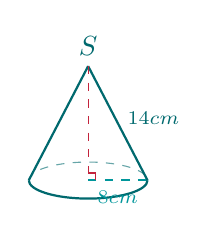
\begin{tikzpicture}[scale=0.58]
          \draw[thick, color=brandNavy] (-1.3, 0) arc (180:360:1.3cm and 0.40cm);
          \draw[dashed, color=brandNavy!60] (-1.3, 0) arc (180:0:1.3cm and 0.40cm);
          \draw[thick, color=brandNavy] (-1.3, 0) -- (0, 2.5) node[above, color=brandNavy] {$S$};
          \draw[thick, color=brandNavy] (1.3, 0) -- (0, 2.5);
          \coordinate (O) at (0,0);
          \coordinate (S) at (0,2.5);
          \draw[dashed, color=brandCrimson] (S) -- (O);
          \draw[dashed, color=brandBlue, thick] (O) -- (1.3, 0) node[midway, below, font=\fontsize{7.5}{7.5}\selectfont] {$8\text{cm}$};
          \node[right, font=\fontsize{7.5}{7.5}\selectfont, color=brandNavy] at (0.65, 1.35) {$14\text{cm}$};
          \draw[color=brandCrimson] (0, 0.16) -- (0.16, 0.16) -- (0.16, 0);
        \end{tikzpicture}\par\vspace{2pt}
        \khlabel{គ}
      \end{minipage}
    \end{center}
    \vspace{-4pt}
    \textbf{គំនូរខាងលើបង្ហាញរូបសូលីតទាំង ៣ ៖} ពីរ៉ាមីតបាតការេ, ពីរ៉ាមីតបាតឆកោណនិយ័ត និងកោន ។
  \end{minipage}\par\vspace{5pt}
\end{multicols}

% =========================================================================
% ចំណុច ១.២ ៖ មាឌនៃសូលីត
% =========================================================================
\khsubsection{១.២}{មាឌនៃសូលីត}

\begin{khcard}
  \textbf{\color{brandNavy}\ding{70} តារាងរូបមន្តមាឌ និងផ្ទៃក្រឡានៃសូលីត ៖}
  \vspace{2pt}
  \begin{center}
    \renewcommand{\arraystretch}{1.15}
    \begin{tabular}{|m{3.8cm}|m{2.6cm}|m{10.8cm}|}
      \hline
      \rowcolor{brandNavy!15}
      \centering\textbf{\color{brandNavy}រូបភាពសូលីត} & 
      \centering\textbf{\color{brandNavy}ឈ្មោះសូលីត} & 
      \centering\arraybackslash\textbf{\color{brandNavy}រូបមន្តមាឌ $V$ និងផ្ទៃក្រឡា} \\
      \hline
      \centering\vspace{2pt}
      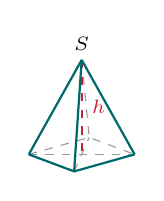
\begin{tikzpicture}[scale=0.48]
        \coordinate (S) at (0, 2.3);
        \coordinate (A) at (-1.4, -0.2);
        \coordinate (B) at (-0.2, -0.65);
        \coordinate (C) at (1.4, -0.2);
        \coordinate (D) at (0.2, 0.25);
        \coordinate (O) at (0, -0.2);
        \draw[dashed, color=gray!80] (A) -- (D) -- (C);
        \draw[dashed, color=gray!80] (S) -- (D);
        \draw[dashed, color=brandCrimson, thick] (S) -- (O) node[midway, right, font=\fontsize{7}{7}\selectfont] {$h$};
        \draw[dashed, color=gray!80] (A) -- (C);
        \draw[dashed, color=gray!80] (B) -- (D);
        \draw[thick, color=brandNavy] (A) -- (B) -- (C);
        \draw[thick, color=brandNavy] (S) -- (A);
        \draw[thick, color=brandNavy] (S) -- (B);
        \draw[thick, color=brandNavy] (S) -- (C);
        \node[above, font=\fontsize{7.5}{7.5}\selectfont] at (S) {$S$};
      \end{tikzpicture}\vspace{2pt} &
      \centering\textbf{\kml ពីរ៉ាមីត} &
      $\bullet$ មាឌ ៖ \koreahl{$V = \frac{1}{3} S_B \times h$} \newline
      - $SO = h$ ជាកម្ពស់នៃពីរ៉ាមីត \quad - $S_B$ ជាផ្ទៃក្រឡាបាត \\
      \hline
      \centering\vspace{2pt}
      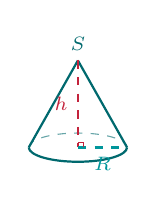
\begin{tikzpicture}[scale=0.48]
        \draw[thick, color=brandNavy] (-1.3, 0) arc (180:360:1.3cm and 0.38cm);
        \draw[dashed, color=brandNavy!60] (-1.3, 0) arc (180:0:1.3cm and 0.38cm);
        \draw[thick, color=brandNavy] (-1.3, 0) -- (0, 2.3) node[above, font=\fontsize{7.5}{7.5}\selectfont] {$S$};
        \draw[thick, color=brandNavy] (1.3, 0) -- (0, 2.3);
        \coordinate (O) at (0,0);
        \coordinate (S) at (0,2.3);
        \draw[dashed, color=brandCrimson, thick] (S) -- (O) node[midway, left, font=\fontsize{7}{7}\selectfont] {$h$};
        \draw[dashed, color=brandBlue, thick] (O) -- (1.3, 0) node[midway, below, font=\fontsize{7}{7}\selectfont] {$R$};
        \draw[color=brandCrimson] (0, 0.14) -- (0.14, 0.14) -- (0.14, 0);
      \end{tikzpicture}\vspace{2pt} &
      \centering\textbf{\kml កោន} &
      $\bullet$ មាឌ ៖ \koreahl{$V = \frac{1}{3} \pi R^2 \times h$} \newline
      - $SO = h$ ជាកម្ពស់កោន \quad - $R$ ជាកាំនៃថាសបាត \\
      \hline
      \centering\vspace{2pt}
      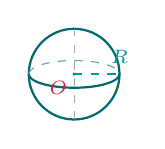
\begin{tikzpicture}[scale=0.48]
        \draw[thick, color=brandNavy] (0,0) circle (1.2cm);
        \draw[thick, color=brandNavy] (-1.2, 0) arc (180:360:1.2cm and 0.36cm);
        \draw[dashed, color=brandNavy!60] (-1.2, 0) arc (180:0:1.2cm and 0.36cm);
        \coordinate (O) at (0,0);
        \fill[brandCrimson] (O) circle (1.2pt) node[below left=-1pt, font=\fontsize{7}{7}\selectfont] {$O$};
        \draw[dashed, color=brandBlue, thick] (O) -- (1.2, 0) node[above, font=\fontsize{7}{7}\selectfont] {$R$};
        \draw[dashed, color=gray!70] (0, -1.2) -- (0, 1.2);
      \end{tikzpicture}\vspace{2pt} &
      \centering\textbf{\kml ស្វ៊ែរ ឬ ប៊ូល} &
      $\bullet$ ផ្ទៃក្រឡាស្វ៊ែរ ៖ \koreahl{$S = 4\pi R^2$} \newline
      $\bullet$ មាឌប៊ូល ៖ \koreahl{$V = \frac{4}{3} \pi R^3$} \newline
      - $O$ ជាផ្ចិតនៃស្វ៊ែរ/ប៊ូល, $R$ ជាកាំ, $D = 2R$ ជាអង្កត់ផ្ចិត \\
      \hline
    \end{tabular}
  \end{center}
\end{khcard}

\begin{multicols}{2}
  % [ស្រួល - Direct calculation: 01..04]
  \noindent\begin{minipage}{\linewidth}
    \exhead{1} គណនាមាឌនៃសូលីតខាងក្រោម ៖
    \begin{center}
      \vspace{-3pt}
      \begin{minipage}[t]{0.32\linewidth}
        \centering
        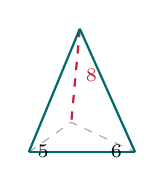
\begin{tikzpicture}[scale=0.54]
          \coordinate (S) at (0, 2.4);
          \coordinate (A) at (-1.2, -0.5);
          \coordinate (B) at (1.3, -0.5);
          \coordinate (C) at (-0.2, 0.2);
          \draw[dashed, color=gray!70] (A) -- (C) -- (B);
          \draw[dashed, color=brandCrimson, thick] (S) -- (C) node[midway, right, font=\fontsize{7}{7}\selectfont] {$8$};
          \draw[thick, color=brandNavy] (A) -- (B);
          \draw[thick, color=brandNavy] (S) -- (A);
          \draw[thick, color=brandNavy] (S) -- (B);
          \node[below left, font=\fontsize{7}{7}\selectfont] at (-0.5, -0.1) {$5$};
          \node[below right, font=\fontsize{7}{7}\selectfont] at (0.5, -0.1) {$6$};
        \end{tikzpicture}\par\vspace{2pt}
        \khlabel{ក}
      \end{minipage}\hfill
      \begin{minipage}[t]{0.32\linewidth}
        \centering
        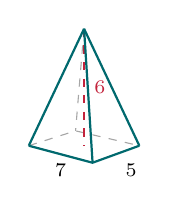
\begin{tikzpicture}[scale=0.54]
          \coordinate (S) at (0, 2.4);
          \coordinate (A) at (-1.3, -0.35);
          \coordinate (B) at (0.2, -0.75);
          \coordinate (C) at (1.3, -0.35);
          \coordinate (D) at (-0.2, 0.0);
          \coordinate (O) at (0, -0.35);
          \draw[dashed, color=gray!70] (A) -- (D) -- (C);
          \draw[dashed, color=gray!70] (S) -- (D);
          \draw[dashed, color=brandCrimson, thick] (S) -- (O) node[midway, right, font=\fontsize{7}{7}\selectfont] {$6$};
          \draw[thick, color=brandNavy] (A) -- (B) -- (C);
          \draw[thick, color=brandNavy] (S) -- (A);
          \draw[thick, color=brandNavy] (S) -- (B);
          \draw[thick, color=brandNavy] (S) -- (C);
          \node[below, font=\fontsize{7}{7}\selectfont] at (-0.55, -0.55) {$7$};
          \node[below right, font=\fontsize{7}{7}\selectfont] at (0.75, -0.55) {$5$};
        \end{tikzpicture}\par\vspace{2pt}
        \khlabel{ខ}
      \end{minipage}\hfill
      \begin{minipage}[t]{0.32\linewidth}
        \centering
        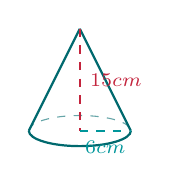
\begin{tikzpicture}[scale=0.54]
          \draw[thick, color=brandNavy] (-1.2, 0) arc (180:360:1.2cm and 0.36cm);
          \draw[dashed, color=brandNavy!60] (-1.2, 0) arc (180:0:1.2cm and 0.36cm);
          \draw[thick, color=brandNavy] (-1.2, 0) -- (0, 2.4);
          \draw[thick, color=brandNavy] (1.2, 0) -- (0, 2.4);
          \draw[dashed, color=brandCrimson, thick] (0, 2.4) -- (0, 0) node[midway, right, font=\fontsize{7}{7}\selectfont] {$15\text{cm}$};
          \draw[dashed, color=brandBlue, thick] (0, 0) -- (1.2, 0) node[midway, below, font=\fontsize{7}{7}\selectfont] {$6\text{cm}$};
        \end{tikzpicture}\par\vspace{2pt}
        \khlabel{គ}
      \end{minipage}
    \end{center}
  \end{minipage}\par\vspace{5pt}

  \noindent\begin{minipage}{\linewidth}
    \exhead{2} ចូររកមាឌកោនដែលមានកម្ពស់ $h$ និងកាំបាត $R$ ក្នុងករណីនីមួយៗខាងក្រោម ៖\par\vspace{3pt}
    \itemtwo{\khlabel{ក} $R = 5\text{cm}, h = 12\text{cm}$}{\khlabel{ខ} $R = 3.4\text{cm}, h = 8.9\text{cm}$}
    \itemtwo{\khlabel{គ} $R = 3.7\text{cm}, h = 7\text{cm}$}{\khlabel{ឃ} $R = 5.2\text{cm}, h = 11\text{cm}$}
    \itemtwo{\khlabel{ង} $R = \sqrt{5}\text{mm}, h = 13.4\text{mm}$}{\khlabel{ច} $R = 7\text{dm}, h = 16\text{dm}$}
  \end{minipage}\par\vspace{5pt}

  \noindent\begin{minipage}{\linewidth}
    \exhead{3} ចូររកផ្ទៃក្រឡាស្វ៊ែរ និងមាឌប៊ូលក្នុងករណីនីមួយៗខាងក្រោម ៖\par\vspace{3pt}
    \itemtwo{\khlabel{ក} $R = 3\text{cm}$}{\khlabel{ខ} $R = 4\text{cm}$}
    \itemtwo{\khlabel{គ} $D = 4\text{cm}$}{\khlabel{ឃ} $D = 12\text{cm}$}
  \end{minipage}\par\vspace{5pt}

  \noindent\begin{minipage}{\linewidth}
    \exhead{4} កោនមួយមានកម្ពស់ $28\text{cm}$ និងកាំនៃថាសបាតមានប្រវែង $13\text{cm}$ ។ ចូរគណនាមាឌកោន គិតជា $\text{dm}^3$ ។
  \end{minipage}\par\vspace{5pt}

  % [មធ្យម - Reverse calculations: 05..09]
  \noindent\begin{minipage}{\linewidth}
    \exhead{5} កោនមួយមានកម្ពស់ $24\text{cm}$ ហើយមានមាឌ $3018\text{cm}^3$ ។ ចូររកផ្ទៃក្រឡាបាតនៃកោននោះ ។
  \end{minipage}\par\vspace{5pt}

  \noindent\begin{minipage}{\linewidth}
    \exhead{6} ពីរ៉ាមីតមួយមានបាតរាងជាចតុកោណកែងមានវិមាត្រ $6\text{cm}$ និង $8\text{cm}$ ។ គេដឹងថាពីរ៉ាមីតនេះមានមាឌស្មើនឹង $3500\text{cm}^3$ ។ ចូរគណនាកម្ពស់នៃពីរ៉ាមីតនោះ ។
  \end{minipage}\par\vspace{5pt}

  \noindent\begin{minipage}{\linewidth}
    \exhead{7} ចូររកកាំស្វ៊ែរដោយស្គាល់ផ្ទៃក្រឡាដូចខាងក្រោម ៖\par\vspace{3pt}
    \itemtwo{\khlabel{ក} $S = \frac{36}{25}\pi\text{cm}^2$}{\khlabel{ខ} $S = \frac{46}{16}\pi\text{m}^2$}
    \vspace{1.5pt}
    \itemtwo{\khlabel{គ} $S = \frac{12}{5}\pi\text{dm}^2$}{\khlabel{ឃ} $S = 1764\pi\text{cm}^2$}
  \end{minipage}\par\vspace{5pt}

  \noindent\begin{minipage}{\linewidth}
    \exhead{8} ចូររកកាំនៃប៊ូលដោយស្គាល់មាឌ ៖\par\vspace{3pt}
    \itemtwo{\khlabel{ក} $V = 288\pi\text{cm}^3$}{\khlabel{ខ} $V = \frac{32}{16}\pi\text{m}^3$}
  \end{minipage}\par\vspace{5pt}

  \noindent\begin{minipage}{\linewidth}
    \exhead{9} ចូររកផ្ទៃក្រឡាស្វ៊ែរ និងមាឌប៊ូលក្នុងករណីនីមួយៗខាងក្រោម ៖\par\vspace{3pt}
    \itemtwo{\khlabel{ក} $R = 3\text{cm}$}{\khlabel{ខ} $D = 18\text{dm}$}
    \itemtwo{\khlabel{គ} $R = 3.7\text{cm}$}{\khlabel{ឃ} $D = 23.2\text{cm}$}
  \end{minipage}\par\vspace{5pt}

  % [ពិបាក - Composite & Inscribed 3D Solids: 10..13]
  \noindent\begin{minipage}{\linewidth}
    \exhead{10} គេឱ្យកោន និងកន្លះស្វ៊ែរដូចរូបខាងក្រោម ៖
    \begin{center}
      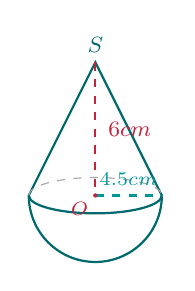
\begin{tikzpicture}[scale=0.65]
        \coordinate (S) at (0, 2.6);
        \coordinate (O) at (0, 0);
        \draw[thick, color=brandNavy] (-1.3, 0) -- (S) node[above, font=\fontsize{8}{8}\selectfont] {$S$} -- (1.3, 0);
        \draw[dashed, color=gray!70] (-1.3, 0) arc (180:0:1.3cm and 0.35cm);
        \draw[color=brandNavy, thick] (-1.3, 0) arc (180:360:1.3cm and 0.35cm);
        \draw[thick, color=brandNavy] (-1.3, 0) arc (180:360:1.3cm);
        \draw[dashed, color=brandCrimson, thick] (S) -- (O) node[midway, right=1pt, font=\fontsize{8}{8}\selectfont] {$6\text{ cm}$};
        \draw[dashed, color=brandBlue, thick] (O) -- (1.3, 0) node[midway, above, font=\fontsize{7.5}{7.5}\selectfont] {$4.5\text{ cm}$};
        \fill[brandCrimson] (O) circle (1.2pt) node[below left=-1pt, font=\fontsize{7.5}{7.5}\selectfont] {$O$};
      \end{tikzpicture}
    \end{center}
    \vspace{-3pt}
    \begin{itemize}[leftmargin=14pt, labelsep=3pt, itemsep=1.5pt]
      \item[\khlabel{ក}] ចូររកមាឌទាំងអស់នៃសូលីត
      \item[\khlabel{ខ}] ចូររកផ្ទៃក្រឡាទាំងអស់នៃសូលីត
    \end{itemize}
  \end{minipage}\par\vspace{5pt}

  \noindent\begin{minipage}{\linewidth}
    \exhead{11} ស៊ីឡាំងមួយមានកាំ $R$ និងកម្ពស់ $h$ គេយកកោនដែលមានកាំ $R$ និងកម្ពស់ $h$ ដាក់ក្នុងស៊ីឡាំងតាមរូប ៖
    \begin{center}
      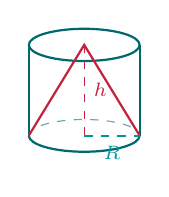
\begin{tikzpicture}[scale=0.64]
        \draw[thick, color=brandNavy] (-1.1, 1.8) arc (180:360:1.1cm and 0.32cm);
        \draw[thick, color=brandNavy] (-1.1, 1.8) arc (180:0:1.1cm and 0.32cm);
        \draw[thick, color=brandNavy] (-1.1, 0) arc (180:360:1.1cm and 0.32cm);
        \draw[dashed, color=brandNavy!60] (-1.1, 0) arc (180:0:1.1cm and 0.32cm);
        \draw[thick, color=brandNavy] (-1.1, 0) -- (-1.1, 1.8);
        \draw[thick, color=brandNavy] (1.1, 0) -- (1.1, 1.8);
        
        \coordinate (S) at (0, 1.8);
        \draw[thick, color=brandCrimson] (-1.1, 0) -- (S) -- (1.1, 0);
        \draw[dashed, color=brandCrimson] (0,0) -- (S) node[midway, right, font=\fontsize{7.5}{7.5}\selectfont] {$h$};
        \draw[dashed, color=brandBlue, thick] (0,0) -- (1.1, 0) node[midway, below, font=\fontsize{7.5}{7.5}\selectfont] {$R$};
      \end{tikzpicture}
    \end{center}
    \vspace{-3pt}
    \begin{itemize}[leftmargin=14pt, labelsep=3pt, itemsep=1.5pt]
      \item[\khlabel{ក}] ចូរគណនាមាឌកោន និងមាឌស៊ីឡាំង ។
      \item[\khlabel{ខ}] ចូរគណនាផលធៀបរវាងមាឌកោន និងមាឌស៊ីឡាំង ។
    \end{itemize}
  \end{minipage}\par\vspace{5pt}

  \noindent\begin{minipage}{\linewidth}
    \exhead{12} កោនមួយមានកាំ $R$ និងកម្ពស់ $h$ ។ នៅក្នុងកោននោះមានស៊ីឡាំងមួយដែលមានរង្វាស់កាំស្មើនឹង $\frac{R}{2}$ ៖
    \begin{center}
      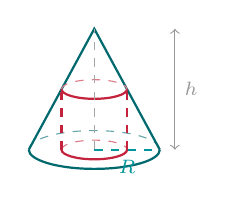
\begin{tikzpicture}[scale=0.64]
        \draw[thick, color=brandNavy] (-1.3, 0) arc (180:360:1.3cm and 0.38cm);
        \draw[dashed, color=brandNavy!60] (-1.3, 0) arc (180:0:1.3cm and 0.38cm);
        \draw[thick, color=brandNavy] (-1.3, 0) -- (0, 2.4) -- (1.3, 0);
        
        \draw[thick, color=brandCrimson] (-0.65, 0) arc (180:360:0.65cm and 0.19cm);
        \draw[dashed, color=brandCrimson!60] (-0.65, 0) arc (180:0:0.65cm and 0.19cm);
        \draw[thick, color=brandCrimson] (-0.65, 1.2) arc (180:360:0.65cm and 0.19cm);
        \draw[dashed, color=brandCrimson!60] (-0.65, 1.2) arc (180:0:0.65cm and 0.19cm);
        \draw[thick, dashed, color=brandCrimson] (-0.65, 0) -- (-0.65, 1.2);
        \draw[thick, dashed, color=brandCrimson] (0.65, 0) -- (0.65, 1.2);
        \draw[dashed, color=gray!70] (0,0) -- (0, 2.4);
        \draw[dashed, color=brandBlue, thick] (0,0) -- (1.3, 0) node[midway, below, font=\fontsize{7.5}{7.5}\selectfont] {$R$};
        \draw[<->, color=gray!80] (1.6, 0) -- (1.6, 2.4) node[midway, right, font=\fontsize{7.5}{7.5}\selectfont] {$h$};
      \end{tikzpicture}
    \end{center}
    \vspace{-3pt}
    \begin{itemize}[leftmargin=14pt, labelsep=3pt, itemsep=1.5pt]
      \item[\khlabel{ក}] ចូរគណនាមាឌនៃស៊ីឡាំងនោះ ។
      \item[\khlabel{ខ}] ចូរគណនាផលធៀបរវាងមាឌស៊ីឡាំង និងមាឌកោន ។
    \end{itemize}
  \end{minipage}\par\vspace{5pt}

  \noindent\begin{minipage}{\linewidth}
    \exhead{13} គូបមួយមានជ្រុង $2a$ នៅក្នុងគូបនោះគេមានស៊ីឡាំងមួយដែលមានកាំស្មើនឹង $a$ និងកម្ពស់ $2a$ ៖
    \begin{center}
      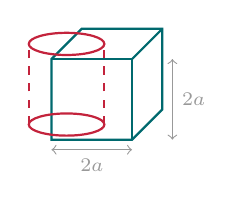
\begin{tikzpicture}[scale=0.64]
        \coordinate (A) at (0,0);
        \coordinate (B) at (1.6,0);
        \coordinate (C) at (2.2, 0.6);
        \coordinate (D) at (0.6, 0.6);
        \coordinate (A1) at (0,1.6);
        \coordinate (B1) at (1.6,1.6);
        \coordinate (C1) at (2.2, 2.2);
        \coordinate (D1) at (0.6, 2.2);
        \draw[thick, color=brandNavy] (A) -- (B) -- (C) -- (C1) -- (D1) -- (A1) -- cycle;
        \draw[thick, color=brandNavy] (B) -- (B1) -- (A1);
        \draw[thick, color=brandNavy] (B1) -- (C1);
        
        \draw[thick, color=brandCrimson] (0.3, 0.3) ellipse (0.75cm and 0.22cm);
        \draw[thick, color=brandCrimson] (0.3, 1.9) ellipse (0.75cm and 0.22cm);
        \draw[thick, dashed, color=brandCrimson] (-0.45, 0.3) -- (-0.45, 1.9);
        \draw[thick, dashed, color=brandCrimson] (1.05, 0.3) -- (1.05, 1.9);
        \draw[<->, color=gray!80] (2.4, 0) -- (2.4, 1.6) node[midway, right, font=\fontsize{7.5}{7.5}\selectfont] {$2a$};
        \draw[<->, color=gray!80] (0, -0.2) -- (1.6, -0.2) node[midway, below, font=\fontsize{7.5}{7.5}\selectfont] {$2a$};
      \end{tikzpicture}
    \end{center}
    \vspace{-3pt}
    \begin{itemize}[leftmargin=14pt, labelsep=3pt, itemsep=1.5pt]
      \item[\khlabel{ក}] ចូរគណនាមាឌនៃស៊ីឡាំង ។
      \item[\khlabel{ខ}] ចូរគណនាផលធៀបរវាងមាឌស៊ីឡាំង និងមាឌគូប ។
    \end{itemize}
  \end{minipage}\par\vspace{5pt}
\end{multicols}

% =========================================================================
% ផ្នែកទី ២ ៖ ផលធៀបផ្ទៃក្រឡានិងមាឌនៃរូបដូចគ្នា
% =========================================================================
\khsection{២}{ផលធៀបផ្ទៃក្រឡានិងមាឌនៃរូបដូចគ្នា}

\khsubsection{២.១}{ផលធៀបផ្ទៃក្រឡានៃរូបដូចគ្នា}

\begin{khboxorange}
  \begin{itemize}[leftmargin=12pt, itemsep=2pt, topsep=1pt, parsep=0pt]
    \item[\color{brandNavy}\ding{228}] \textbf{កាលណារូបធរណីមាត្រពីរដូចគ្នា ផលធៀបរវាងផ្ទៃក្រឡាស្មើនឹងការ៉េនៃផលធៀបរវាងធាតុត្រូវគ្នាពីរ ៖}
    \begin{equation*}
      \koreahl{$\frac{S_1}{S_2} = \left(\frac{a_1}{a_2}\right)^2 = k^2$} \quad \text{($k$ ជាផលធៀបដូចគ្នា ឬផលធៀបវិមាត្រត្រូវគ្នា)}
    \end{equation*}
    \item[\color{brandCrimson}\ding{228}] បើផលធៀបវិមាត្រត្រូវគ្នាគឺ $k = \frac{a_1}{a_2}$ នោះផលធៀបបរិមាត្រគឺ $\frac{P_1}{P_2} = k$ ហើយផលធៀបផ្ទៃក្រឡាគឺ $\frac{S_1}{S_2} = k^2$ ។
  \end{itemize}
\end{khboxorange}

\begin{multicols}{2}
  % [ស្រួល - Fundamental visual concepts: 01..03]
  \noindent\begin{minipage}{\linewidth}
    \exhead{1} គេមានការ៉េ $A$ និងការ៉េ $B$ ជារូបដូចគ្នា ៖
    \begin{center}
      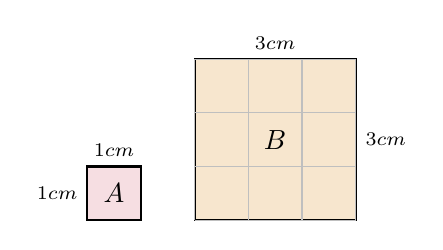
\begin{tikzpicture}[scale=0.62]
        \draw[thick, fill=brandCrimson!15] (0,0) rectangle (1.1, 1.1);
        \node at (0.55, 0.55) {$A$};
        \node[above, font=\fontsize{7.5}{7.5}\selectfont] at (0.55, 1.1) {$1\text{cm}$};
        \node[left, font=\fontsize{7.5}{7.5}\selectfont] at (0, 0.55) {$1\text{cm}$};
        
        \draw[thick, fill=brandGold!20] (2.2,0) rectangle (5.5, 3.3);
        \draw[step=1.1, gray!50, thin] (2.2,0) grid (5.5, 3.3);
        \node at (3.85, 1.65) {$B$};
        \node[above, font=\fontsize{7.5}{7.5}\selectfont] at (3.85, 3.3) {$3\text{cm}$};
        \node[right, font=\fontsize{7.5}{7.5}\selectfont] at (5.5, 1.65) {$3\text{cm}$};
      \end{tikzpicture}
    \end{center}
    \vspace{-3pt}
    $\bullet$ ផ្ទៃក្រឡាការ៉េ $A$ គឺ $1 \times 1 = 1\text{cm}^2$ \newline
    $\bullet$ ផ្ទៃក្រឡាការ៉េ $B$ គឺ $3 \times 3 = 9\text{cm}^2$ \newline
    $\implies$ ផលធៀបផ្ទៃក្រឡា ៖ $\frac{S_A}{S_B} = \frac{1}{9} = \left(\frac{1}{3}\right)^2$ ។
  \end{minipage}\par\vspace{5pt}

  \noindent\begin{minipage}{\linewidth}
    \exhead{2} ចតុកោណកែងពីរដូចគ្នា $C$ និង $D$ ៖
    \begin{center}
      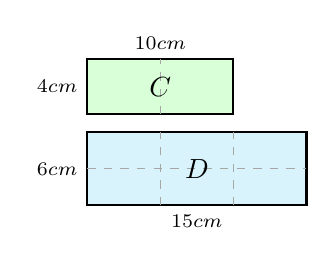
\begin{tikzpicture}[scale=0.58]
        \draw[thick, fill=green!15] (0, 2.0) rectangle (3.2, 3.2);
        \draw[dashed, color=gray!70] (1.6, 2.0) -- (1.6, 3.2);
        \node at (1.6, 2.6) {$C$};
        \node[left, font=\fontsize{7}{7}\selectfont] at (0, 2.6) {$4\text{cm}$};
        \node[above, font=\fontsize{7}{7}\selectfont] at (1.6, 3.2) {$10\text{cm}$};
        
        \draw[thick, fill=cyan!15] (0, 0) rectangle (4.8, 1.6);
        \draw[dashed, color=gray!70] (1.6, 0) -- (1.6, 1.6);
        \draw[dashed, color=gray!70] (3.2, 0) -- (3.2, 1.6);
        \draw[dashed, color=gray!70] (0, 0.8) -- (4.8, 0.8);
        \node at (2.4, 0.8) {$D$};
        \node[left, font=\fontsize{7}{7}\selectfont] at (0, 0.8) {$6\text{cm}$};
        \node[below, font=\fontsize{7}{7}\selectfont] at (2.4, 0) {$15\text{cm}$};
      \end{tikzpicture}
    \end{center}
    \vspace{-3pt}
    $\bullet$ ផលធៀបបណ្ដោយ ៖ $\frac{15}{10} = \frac{3}{2}$ \newline
    $\bullet$ ផលធៀបទទឹង ៖ $\frac{6}{4} = \frac{3}{2}$ \newline
    $\bullet$ ផលធៀបផ្ទៃក្រឡា ៖ $\frac{15 \times 6}{10 \times 4} = \frac{3 \times 3}{2 \times 2} = \left(\frac{3}{2}\right)^2$ ។
  \end{minipage}\par\vspace{5pt}

  \noindent\begin{minipage}{\linewidth}
    \exhead{3} ចូរសរសេរផលធៀបបរិមាត្រ និងផលធៀបផ្ទៃក្រឡានៃរូបខាងក្រោម ៖
    \begin{center}
      \vspace{-3pt}
      \begin{minipage}[t]{0.48\linewidth}
        \centering
        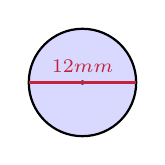
\begin{tikzpicture}[scale=0.62]
          \draw[thick, fill=blue!15] (0,0) circle (1.1cm);
          \fill (0,0) circle (1.3pt);
          \draw[thick, color=brandCrimson] (-1.1, 0) -- (1.1, 0) node[midway, above, font=\fontsize{7}{7}\selectfont] {$12\text{mm}$};
        \end{tikzpicture}\par\vspace{2pt}
        \khlabel{ក}
      \end{minipage}\hfill
      \begin{minipage}[t]{0.48\linewidth}
        \centering
        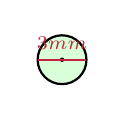
\begin{tikzpicture}[scale=0.62]
          \draw[thick, fill=green!15] (0,0) circle (0.5cm);
          \fill (0,0) circle (1.3pt);
          \draw[thick, color=brandCrimson] (-0.5, 0) -- (0.5, 0) node[midway, above, font=\fontsize{7.5}{7.5}\selectfont] {$3\text{mm}$};
        \end{tikzpicture}\par\vspace{2pt}
        \khlabel{ខ}
      \end{minipage}
    \end{center}
  \end{minipage}\par\vspace{5pt}

  % [មធ្យម - Area Ratios & Scaling: 04..08]
  \noindent\begin{minipage}{\linewidth}
    \exhead{4} ត្រីកោណទាំងពីរខាងស្ដាំនេះជាត្រីកោណដូចគ្នា ។ ចូររកផ្ទៃក្រឡាត្រីកោណ $S$ ៖
    \begin{center}
      \vspace{-5pt}
      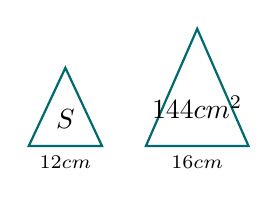
\begin{tikzpicture}[scale=0.62]
        \draw[thick, color=brandNavy] (0, 0) -- (1.5, 0) -- (0.75, 1.6) -- cycle;
        \node at (0.75, 0.55) {$S$};
        \node[below, font=\fontsize{7.5}{7.5}\selectfont] at (0.75, 0) {$12\text{cm}$};
        
        \draw[thick, color=brandNavy] (2.4, 0) -- (4.5, 0) -- (3.45, 2.4) -- cycle;
        \node at (3.45, 0.8) {$144\text{cm}^2$};
        \node[below, font=\fontsize{7.5}{7.5}\selectfont] at (3.45, 0) {$16\text{cm}$};
      \end{tikzpicture}
    \end{center}
  \end{minipage}\par\vspace{5pt}

  \noindent\begin{minipage}{\linewidth}
    \exhead{5} គេមានចតុកោណកែងពីរដូចគ្នាដែលមានផ្ទៃក្រឡារៀងគ្នា $18\text{dm}^2$ និង $8\text{dm}^2$ ។ គណនាបណ្ដោយចតុកោណកែងធំ បើចតុកោណកែងតូចមានបណ្ដោយ $6\text{dm}$ ។
  \end{minipage}\par\vspace{5pt}

  \noindent\begin{minipage}{\linewidth}
    \exhead{6} គេមានចតុកោណកែងពីរដូចគ្នាដែលមានផ្ទៃក្រឡារៀងគ្នា $30\text{m}^2$ និង $20\text{m}^2$ ។ គណនាទទឹងនៃចតុកោណកែងតូច បើចតុកោណកែងធំមានទទឹង $5\text{m}$ ។
  \end{minipage}\par\vspace{5pt}

  \noindent\begin{minipage}{\linewidth}
    \exhead{7} រូបថតនៃជញ្ជាំងមួយមានកម្ពស់ $3\text{cm}$ និងមានផ្ទៃក្រឡាស្មើនឹង $9\text{cm}^2$ ។ គេដឹងថាជញ្ជាំងមានកម្ពស់ពិត $6\text{m}$ ។ តើវាមានផ្ទៃក្រឡាពិតប្រាកដប៉ុន្មាន $\text{m}^2$ ?
  \end{minipage}\par\vspace{5pt}

  \noindent\begin{minipage}{\linewidth}
    \exhead{8} ផ្ទៃក្រឡានៃទីធ្លាសាលាមួយមានរង្វាស់ $144\text{cm}^2$ នៅក្នុងផែនទីទីមួយ ហើយមានរង្វាស់ស្មើនឹង $256\text{cm}^2$ នៅក្នុងផែនទីទីពីរ ។ ដោយដឹងថាវិមាត្រមួយនៃទីធ្លានោះស្មើនឹង $18\text{cm}$ នៅក្នុងផែនទីទីមួយ ។ តើវិមាត្រនេះស្មើនឹងប៉ុន្មាន $\text{cm}$ នៅក្នុងផែនទីទីពីរ ?
  \end{minipage}\par\vspace{5pt}

  % [ពិបាក - Advanced Geometry Ratios: 09..13]
  \noindent\begin{minipage}{\linewidth}
    \exhead{9} គេឱ្យ $AB \parallel CD$ ដែល $\frac{BE}{CE} = \frac{1}{2}$ ។ ផ្ទៃក្រឡា $\Delta CED = 16\text{cm}^2$ ។ ចូររកផ្ទៃក្រឡា $\Delta AEB$ ៖
    \begin{center}
      \vspace{-5pt}
      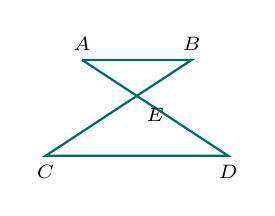
\begin{tikzpicture}[scale=0.58]
        \coordinate (A) at (-1.2, 1.2);
        \coordinate (B) at (1.2, 1.2);
        \coordinate (C) at (-2.0, -0.9);
        \coordinate (D) at (2.0, -0.9);
        \coordinate (E) at (0, 0);
        \draw[thick, color=brandNavy] (A) -- (B) -- (C) -- (D) -- (A);
        \node[above, font=\fontsize{7.5}{7.5}\selectfont] at (A) {$A$};
        \node[above, font=\fontsize{7.5}{7.5}\selectfont] at (B) {$B$};
        \node[below, font=\fontsize{7.5}{7.5}\selectfont] at (C) {$C$};
        \node[below, font=\fontsize{7.5}{7.5}\selectfont] at (D) {$D$};
        \node[right, font=\fontsize{7.5}{7.5}\selectfont] at (E) {$E$};
      \end{tikzpicture}
    \end{center}
  \end{minipage}\par\vspace{5pt}

  \noindent\begin{minipage}{\linewidth}
    \exhead{10} តាមរូបខាងស្ដាំ តើផ្ទៃក្រឡាការ៉េ $DEFG$ តូចជាងផ្ទៃក្រឡាការ៉េ $ABCD$ ប៉ុន្មានដង ?
    \begin{center}
      \vspace{-5pt}
      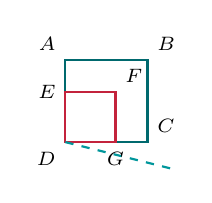
\begin{tikzpicture}[scale=0.58]
        \draw[thick, color=brandNavy] (0,0) coordinate (D) -- (1.8,0) coordinate (C) -- (1.8,1.8) coordinate (B) -- (0,1.8) coordinate (A) -- cycle;
        \draw[thick, color=brandCrimson] (0,0) -- (1.1, 0) coordinate (G) -- (1.1, 1.1) coordinate (F) -- (0, 1.1) coordinate (E) -- cycle;
        \draw[thick, dashed, color=brandBlue] (0, 0) -- (2.4, -0.6);
        \node[above left, font=\fontsize{7.5}{7.5}\selectfont] at (A) {$A$};
        \node[above right, font=\fontsize{7.5}{7.5}\selectfont] at (B) {$B$};
        \node[above right, font=\fontsize{7.5}{7.5}\selectfont] at (C) {$C$};
        \node[below left, font=\fontsize{7.5}{7.5}\selectfont] at (D) {$D$};
        \node[left, font=\fontsize{7.5}{7.5}\selectfont] at (E) {$E$};
        \node[above right, font=\fontsize{7.5}{7.5}\selectfont] at (F) {$F$};
        \node[below, font=\fontsize{7.5}{7.5}\selectfont] at (G) {$G$};
      \end{tikzpicture}
    \end{center}
  \end{minipage}\par\vspace{5pt}

  \noindent\begin{minipage}{\linewidth}
    \exhead{11} គេឱ្យប្រលេឡូក្រាម $ABCD$ និង $I$ ជាចំណុចកណ្ដាលនៃ $AB$ ។ បន្ទាត់ $BD$ និង $CI$ ប្រសព្វគ្នាត្រង់ $O$ ។ តើផ្ទៃក្រឡា $\Delta BIO$ តូចជាងផ្ទៃក្រឡា $\Delta DOC$ ប៉ុន្មានដង ?
    \begin{center}
      \vspace{-5pt}
      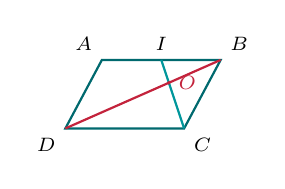
\begin{tikzpicture}[scale=0.58]
        \coordinate (D) at (0,0);
        \coordinate (C) at (2.6,0);
        \coordinate (A) at (0.8, 1.5);
        \coordinate (B) at (3.4, 1.5);
        \coordinate (I) at ($(A)!0.5!(B)$);
        \draw[thick, color=brandNavy] (A) -- (B) -- (C) -- (D) -- cycle;
        \draw[thick, color=brandCrimson] (B) -- (D);
        \draw[thick, color=brandBlue] (C) -- (I);
        \coordinate (O) at (intersection of B--D and C--I);
        \fill[brandCrimson] (O) circle (1.2pt) node[right, font=\fontsize{7.5}{7.5}\selectfont] {$O$};
        \node[above left, font=\fontsize{7.5}{7.5}\selectfont] at (A) {$A$};
        \node[above right, font=\fontsize{7.5}{7.5}\selectfont] at (B) {$B$};
        \node[below right, font=\fontsize{7.5}{7.5}\selectfont] at (C) {$C$};
        \node[below left, font=\fontsize{7.5}{7.5}\selectfont] at (D) {$D$};
        \node[above, font=\fontsize{7.5}{7.5}\selectfont] at (I) {$I$};
      \end{tikzpicture}
    \end{center}
  \end{minipage}\par\vspace{5pt}

  \noindent\begin{minipage}{\linewidth}
    \exhead{12} ទីធ្លាមួយមានផ្ទៃក្រឡាពិត $9600\text{m}^2$ ។ តើផ្ទៃក្រឡានេះមានប៉ុន្មាន $\text{cm}^2$ នៅក្នុងប្លង់មួយដែលមានមាត្រដ្ឋាន $\frac{1}{2500}$ ?
  \end{minipage}\par\vspace{5pt}

  \noindent\begin{minipage}{\linewidth}
    \exhead{13} ផ្ទៃក្រឡានៃត្រីកោណសម័ង្សដែលមានជ្រុង $1\text{cm}$ ។ តើត្រូវជាប៉ុន្មានភាគរយនៃផ្ទៃក្រឡានៃការ៉េដែលមានរង្វាស់ជ្រុង $1\text{cm}$ ?
    \begin{center}
      \vspace{-5pt}
      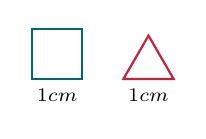
\begin{tikzpicture}[scale=0.58]
        \draw[thick, color=brandNavy] (0,0) rectangle (1.1, 1.1);
        \node[below, font=\fontsize{7.5}{7.5}\selectfont] at (0.55, 0) {$1\text{cm}$};
        \draw[thick, color=brandCrimson] (2.0, 0) -- (3.1, 0) -- (2.55, 0.95) -- cycle;
        \node[below, font=\fontsize{7.5}{7.5}\selectfont] at (2.55, 0) {$1\text{cm}$};
      \end{tikzpicture}
    \end{center}
  \end{minipage}\par\vspace{5pt}
\end{multicols}

% =========================================================================
% ចំណុច ២.២ ៖ ផលធៀបមាឌនៃសូលីតដូចគ្នា
% =========================================================================
\khsubsection{២.២}{ផលធៀបមាឌនៃសូលីតដូចគ្នា}

\begin{khboxorange}
  \begin{itemize}[leftmargin=12pt, itemsep=2pt, topsep=1pt, parsep=0pt]
    \item[\color{brandNavy}\ding{228}] \textbf{កាលណាសូលីតពីរដូចគ្នា ផលធៀបរវាងមាឌស្មើនឹងគូបនៃផលធៀបរវាងធាតុត្រូវគ្នាពីរ ៖}
    \begin{equation*}
      \koreahl{$\frac{V_1}{V_2} = \left(\frac{a_1}{a_2}\right)^3 = k^3$} \quad \text{($k$ ជាផលធៀបវិមាត្រត្រូវគ្នា)}
    \end{equation*}
    \item[\color{brandCrimson}\ding{228}] \textbf{ទំនាក់ទំនងសង្ខេប ៖} $\frac{a_1}{a_2} = k \implies \frac{S_1}{S_2} = k^2 \implies \frac{V_1}{V_2} = k^3$
  \end{itemize}
\end{khboxorange}

\begin{multicols}{2}
  % [ស្រួល - Fundamental Volume Concepts: 01, 02]
  \noindent\begin{minipage}{\linewidth}
    \exhead{1} គេមានគូបពីរជារូបដូចគ្នា ៖
    \begin{center}
      \vspace{-5pt}
      \begin{tikzpicture}[scale=0.54]
        \coordinate (A) at (0,0);
        \coordinate (B) at (0.85,0);
        \coordinate (C) at (1.25, 0.35);
        \coordinate (D) at (0.4, 0.35);
        \coordinate (A1) at (0,0.85);
        \coordinate (B1) at (0.85,0.85);
        \coordinate (C1) at (1.25, 1.2);
        \coordinate (D1) at (0.4, 1.2);
        \draw[thick, color=brandNavy] (A) -- (B) -- (C) -- (C1) -- (D1) -- (A1) -- cycle;
        \draw[thick, color=brandNavy] (B) -- (B1) -- (A1);
        \draw[thick, color=brandNavy] (B1) -- (C1);
        \node[below, font=\fontsize{7}{7}\selectfont] at (0.42, 0) {$1\text{cm}$};
        \node[below=1pt, font=\fontsize{7.5}{7.5}\selectfont\kml] at (0.6, -0.3) {រូប (a)};
        
        \coordinate (E) at (2.6,0);
        \coordinate (F) at (4.3,0);
        \coordinate (G) at (5.15, 0.65);
        \coordinate (H) at (3.45, 0.65);
        \coordinate (E1) at (2.6,1.7);
        \coordinate (F1) at (4.3,1.7);
        \coordinate (G1) at (5.15, 2.35);
        \coordinate (H1) at (3.45, 2.35);
        \draw[thick, color=brandCrimson] (E) -- (F) -- (G) -- (G1) -- (H1) -- (E1) -- cycle;
        \draw[thick, color=brandCrimson] (F) -- (F1) -- (E1);
        \draw[thick, color=brandCrimson] (F1) -- (G1);
        \draw[dashed, color=gray!60] (3.45,0) -- (3.45,1.7) -- (4.3, 2.05);
        \draw[dashed, color=gray!60] (2.6,0.85) -- (4.3,0.85) -- (5.15, 1.5);
        \node[below, font=\fontsize{7}{7}\selectfont] at (3.45, 0) {$2\text{cm}$};
        \node[below=1pt, font=\fontsize{7.5}{7.5}\selectfont\kml] at (3.85, -0.3) {រូប (b)};
      \end{tikzpicture}
    \end{center}
    \vspace{-3pt}
    $\bullet$ មាឌគូប (a) ៖ $V_a = 1 \times 1 \times 1 = 1\text{cm}^3$ \newline
    $\bullet$ មាឌគូប (b) ៖ $V_b = 2 \times 2 \times 2 = 8\text{cm}^3$ \newline
    $\implies$ ផលធៀបមាឌ ៖ $\frac{V_a}{V_b} = \frac{1}{8} = \left(\frac{1}{2}\right)^3$ ។
  \end{minipage}\par\vspace{5pt}

  \noindent\begin{minipage}{\linewidth}
    \exhead{2} ប្រអប់ពីរដូចគ្នា (វិមាត្រ $10 \times 8 \times 6$ និង $15 \times 12 \times 9$) ៖
    \begin{itemize}[leftmargin=12pt, labelsep=2pt, itemsep=0.5pt, topsep=1pt]
      \item ផលធៀបបណ្ដោយ ៖ $\frac{15}{10} = \frac{3}{2}$ \quad ផលធៀបទទឹង ៖ $\frac{12}{8} = \frac{3}{2}$
      \item ផលធៀបកម្ពស់ ៖ $\frac{9}{6} = \frac{3}{2}$
    \end{itemize}
    $\implies$ ផលធៀបមាឌ ៖ $\frac{V_1}{V_2} = \frac{15 \times 12 \times 9}{10 \times 8 \times 6} = \left(\frac{3}{2}\right)^3$ ។
  \end{minipage}\par\vspace{5pt}

  % [មធ្យម - Geometric Volume Proportions: 03..07]
  \noindent\begin{minipage}{\linewidth}
    \exhead{3} ផលធៀបរវាងផ្ទៃក្រឡាទាំងអស់នៃគូបស្មើនឹង $\frac{16}{25}$ ។ ចូរគណនាផលធៀបរវាងជ្រុង និងផលធៀបរវាងមាឌនៃគូបពីរដូចគ្នា ។
  \end{minipage}\par\vspace{5pt}

  \noindent\begin{minipage}{\linewidth}
    \exhead{4} ផលធៀបរវាងបណ្ដោយនៃប្រលេពីប៉ែតកែងដូចគ្នាពីរស្មើនឹង $\frac{4}{3}$ ។ បើប្រលេពីប៉ែតកែងតូចមានមាឌ $54\text{dm}^3$ ចូររកមាឌប្រលេពីប៉ែតកែងធំ ។
  \end{minipage}\par\vspace{5pt}

  \noindent\begin{minipage}{\linewidth}
    \exhead{5} តាមរូបខាងស្ដាំ គេឱ្យមាឌនៃប្រលេពីប៉ែតកែងធំស្មើនឹង $216\text{m}^3$ និងប្រលេពីប៉ែតកែងតូចមានមាឌ $64\text{m}^3$ ។ ចូរគណនាបណ្ដោយនៃប្រលេពីប៉ែតធំ $x$ (បើបណ្ដោយតូច $6\text{m}$) ៖
    \begin{center}
      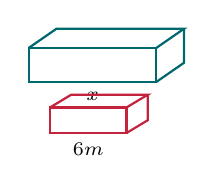
\begin{tikzpicture}[scale=0.54]
        \draw[thick, color=brandNavy] (0, 1.2) rectangle (3.0, 2.0);
        \draw[thick, color=brandNavy] (0, 2.0) -- (0.65, 2.45) -- (3.65, 2.45) -- (3.0, 2.0);
        \draw[thick, color=brandNavy] (3.65, 2.45) -- (3.65, 1.65) -- (3.0, 1.2);
        \node[below, font=\fontsize{7.5}{7.5}\selectfont] at (1.5, 1.2) {$x$};
        
        \draw[thick, color=brandCrimson] (0.5, 0) rectangle (2.3, 0.6);
        \draw[thick, color=brandCrimson] (0.5, 0.6) -- (1.0, 0.9) -- (2.8, 0.9) -- (2.3, 0.6);
        \draw[thick, color=brandCrimson] (2.8, 0.9) -- (2.8, 0.3) -- (2.3, 0);
        \node[below, font=\fontsize{7.5}{7.5}\selectfont] at (1.4, 0) {$6\text{m}$};
      \end{tikzpicture}
    \end{center}
  \end{minipage}\par\vspace{5pt}

  \noindent\begin{minipage}{\linewidth}
    \exhead{6} គេឱ្យ $DE \parallel BC$, $AD = 3\text{cm}, AB = 5\text{cm}$ ហើយផ្ទៃក្រឡា $\Delta ADE = 6\text{cm}^2$ ៖
    \begin{center}
      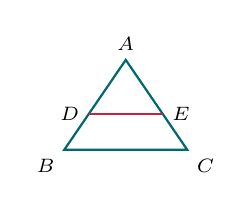
\begin{tikzpicture}[scale=0.60]
        \coordinate (A) at (0, 1.9);
        \coordinate (B) at (-1.3, 0);
        \coordinate (C) at (1.3, 0);
        \coordinate (D) at ($(A)!0.6!(B)$);
        \coordinate (E) at ($(A)!0.6!(C)$);
        \draw[thick, color=brandNavy] (A) -- (B) -- (C) -- cycle;
        \draw[thick, color=brandCrimson] (D) -- (E);
        \node[above, font=\fontsize{7.5}{7.5}\selectfont] at (A) {$A$};
        \node[below left, font=\fontsize{7.5}{7.5}\selectfont] at (B) {$B$};
        \node[below right, font=\fontsize{7.5}{7.5}\selectfont] at (C) {$C$};
        \node[left, font=\fontsize{7.5}{7.5}\selectfont] at (D) {$D$};
        \node[right, font=\fontsize{7.5}{7.5}\selectfont] at (E) {$E$};
      \end{tikzpicture}
    \end{center}
    \vspace{-3pt}
    \begin{itemize}[leftmargin=14pt, labelsep=3pt, itemsep=1.5pt]
      \item[\khlabel{ក}] ចូររកផ្ទៃក្រឡាត្រីកោណ $ABC$
      \item[\khlabel{ខ}] ចូររកផ្ទៃក្រឡាចតុកោណ $DECB$
    \end{itemize}
  \end{minipage}\par\vspace{5pt}

  \noindent\begin{minipage}{\linewidth}
    \exhead{7} ផលធៀបផ្ទៃក្រឡាទាំងអស់នៃគូបពីរស្មើនឹង $16 : 25$ ។ តើគូបធំមានម៉ាសប៉ុន្មានបើគូបតូចមានម៉ាស $32\text{g}$ (គូបទាំងពីរធ្វើពីវត្ថុធាតុតែមួយ និងជាគូបដូចគ្នា) ?
  \end{minipage}\par\vspace{5pt}

  % [ពិបាក - Truncated Solids & Word Problems: 08..11]
  \noindent\begin{minipage}{\linewidth}
    \exhead{8} គេកាត់កោនឱ្យស្របនឹងបាតជាបីចំណែក (ដូចរូបខាងស្ដាំ) ។ មុខកាត់មានអង្កត់ផ្ចិតរៀងគ្នា $6\text{cm}$ និង $10\text{cm}$ និងកម្ពស់រៀងគ្នា $x, 4\text{cm}, 2\text{cm}$ ៖
    \begin{center}
      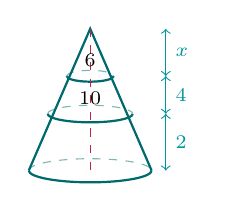
\begin{tikzpicture}[scale=0.60]
        \draw[thick, color=brandNavy] (-0.5, 2.0) arc (180:360:0.5cm and 0.12cm);
        \draw[dashed, color=brandNavy!50] (-0.5, 2.0) arc (180:0:0.5cm and 0.12cm);
        \draw[thick, color=brandNavy] (-0.9, 1.2) arc (180:360:0.9cm and 0.18cm);
        \draw[dashed, color=brandNavy!50] (-0.9, 1.2) arc (180:0:0.9cm and 0.18cm);
        \draw[thick, color=brandNavy] (-1.3, 0) arc (180:360:1.3cm and 0.25cm);
        \draw[dashed, color=brandNavy!50] (-1.3, 0) arc (180:0:1.3cm and 0.25cm);
        \draw[thick, color=brandNavy] (-1.3, 0) -- (0, 3.0) -- (1.3, 0);
        \draw[dashed, color=brandCrimson] (0, 3.0) -- (0, 0);
        \draw[<->, color=brandBlue] (1.6, 2.0) -- (1.6, 3.0) node[midway, right, font=\fontsize{7}{7}\selectfont] {$x$};
        \draw[<->, color=brandBlue] (1.6, 1.2) -- (1.6, 2.0) node[midway, right, font=\fontsize{7}{7}\selectfont] {$4$};
        \draw[<->, color=brandBlue] (1.6, 0) -- (1.6, 1.2) node[midway, right, font=\fontsize{7}{7}\selectfont] {$2$};
        \node[above, font=\fontsize{7}{7}\selectfont] at (0, 2.0) {$6$};
        \node[above, font=\fontsize{7}{7}\selectfont] at (0, 1.2) {$10$};
      \end{tikzpicture}
    \end{center}
    \vspace{-3pt}
    \begin{itemize}[leftmargin=14pt, labelsep=3pt, itemsep=1.5pt]
      \item[\khlabel{ក}] ចូរគណនា $x$
      \item[\khlabel{ខ}] ចូររកមាឌនៃកោននោះ
    \end{itemize}
  \end{minipage}\par\vspace{5pt}

  \columnbreak

  \noindent\begin{minipage}{\linewidth}
    \exhead{9} $SABCD$ ជាពីរ៉ាមីតដែលមានបាតជាការេមានជ្រុង $60\text{cm}$ ។ កម្ពស់ $[SO] = 80\text{cm}$ ។ គេកាត់ពីរ៉ាមីតនេះឱ្យស្របនឹងបាត បានការេ $EFGK$ ។ គេឱ្យ $OO' = x$ ៖
    \begin{itemize}[leftmargin=14pt, labelsep=3pt, itemsep=1.5pt]
      \item[\khlabel{ក}] ចូររកជ្រុងនៃការេ $EFGK$ តាមតម្លៃ $x$
      \item[\khlabel{ខ}] បើ $x = 30\text{cm}$ គណនាមាឌនៃកំណាត់ពីរ៉ាមីតខណ្ឌដោយ $ABCD$ និង $EFGK$ ។
    \end{itemize}
  \end{minipage}\par\vspace{5pt}

  \noindent\begin{minipage}{\linewidth}
    \exhead{10} អ្នកលក់ឪឡឹកម្នាក់កំណត់លក់ផ្លែឪឡឹកតូចពីរថ្លៃស្មើនឹងផ្លែឪឡឹកធំមួយ ។ ដោយដឹងថាកាំនៃផ្លែឪឡឹកតូចស្មើនឹង $\frac{1}{4}$ នៃកាំផ្លែឪឡឹកធំ ។ តើអ្នកទិញគួរជ្រើសរើសមួយណាដើម្បីបានចំណេញជាង ?
  \end{minipage}\par\vspace{5pt}

  \noindent\begin{minipage}{\linewidth}
    \exhead{11} ឈ្មួញម្នាក់លក់ម៉ាស៊ីនបោកខោអាវ ពីរប្រភេទដែលមានរាងស៊ីឡាំងដូចគ្នា ។ តែវិមាត្រនៃម៉ាស៊ីនទីមួយស្មើនឹង $\frac{9}{10}$ នៃវិមាត្រម៉ាស៊ីនទីពីរ ។ ឯតម្លៃនៃម៉ាស៊ីនតូចស្មើនឹង $\frac{7}{10}$ នៃម៉ាស៊ីនធំ ។ តើគេត្រូវជ្រើសរើសយកម៉ាស៊ីនប្រភេទណាទើបចំណេញជាង ?
  \end{minipage}\par\vspace{5pt}
\end{multicols}

\vspace{6pt}
\noindent
\begin{tcolorbox}[
  enhanced,
  colframe=brandNavy!50,
  colback=brandTealBg,
  boxrule=0.7pt,
  arc=5pt,
  halign=center,
  valign=center,
  top=4pt, bottom=4pt
]
  \fontsize{10}{10}\selectfont\kml\bfseries\color{brandCrimson}
  \ding{72}\ ព្យាយាមគង់បានសម្រេច \ding{72}
\end{tcolorbox}

\end{document}
